\section{Auswertung}
\label{sec:Auswertung}

Die in \autoref{sec:Auswertung} gezeigten Grafiken und Ausgleichsrechnungen sind mithilfe der Python-Bibliotheken Matplotlib \cite{matplotlib}, Scipy \cite{scipy} und Numpy \cite{numpy}
erstellt worden.

\subsection{Bestimmung der Zeitkonstante eines RC Glieds mit angelegter Rechteckspannung}
\label{sec:4.1}
\begin{table}[H]
    \centering
    \caption{Abgelesene Kondensatorspannung in Abhängigkeit der Zeit.}
    \begin{tabular}{
      S[table-format=4.0]
      S[table-format=2.3]
    }
      \toprule
      {$t\left[\unit{ms}\right]$} & {$U_C\left[\unit{V}\right]$}\\
      \midrule
      0.0 & 4.00 \\
      0.4 & 3.40\\
      0.8 & 3.00\\
      1.2 & 2.50\\
      1.6 & 2.20\\
      2.0 & 1.90\\
      2.4 & 1.70\\
      2.8 & 1.40\\
      3.2 & 1.30\\
      3.6 & 1.10\\
      4.0 & 0.90\\
      4.4 & 0.80\\
      4.8 & 0.70\\
      5.2 & 0.60\\
      5.6 & 0.50\\
      6.0 & 0.40\\
      6.4 & 0.40\\
      6.8 & 0.35\\
      7.2 & 0.30\\
      7.6 & 0.25\\
      8.0 & 0.23\\
      8.4 & 0.20\\
      8.8 & 0.20\\
      9.2 & 0.17\\
      9.6 & 0.15\\
      10.0& 0.10\\
      12.0 & 0.00\\
      \bottomrule
  \end{tabular}
  \end{table}  

Die gemessenen Werte können nun als Funktion von $t$ dargestellt werden. Wird der ln$(\frac{U_C}{U_0})$ gegen $t$ aufgetragen, so entsteht \autoref{rc_graph}.
\begin{figure}[H]
    \includegraphics[width=\linewidth]{build/entladekurve.pdf}
    \caption{Amplitudenverhältnis $\frac{U_C}{U_0}$ logarithmisch gegen die Zeit $t$ aufgetragen.}
    \label{rc_graph}
\end{figure} 
Durch eine lineare Ausgleichsrechnung wird die Funktion
\begin{equation*}
    f(x) = ax + b
\end{equation*}
an die Messwerte gefittet. Mit der Python Bibliothek SciPy \cite{scipy} ergibt sich für die Koeffizienten $a = \SI{-0.351(0.004)}{\frac{1}{ms}}$ und $b = -0.04 \pm 0.02$.
Mit dem Zusammenhang 
\begin{equation*}
    \ln{\frac{U_C}{U_0}} = - \frac{t}{RC}
\end{equation*}
lässt sich $RC$ zu $RC = -\frac{1}{a}$ bestimmen, wobei $a$ die Steigung der Ausgleichsgeraden ist. Dadurch ergibt sich für die Zeitkonstante
\begin{equation*}
    RC = -\frac{1}{a} = \SI{2.849(0.032)}{ms}.
\end{equation*}

\subsection{Bestimmung der Zeitkonstante mit angelegter Sinusspannung}
\label{sec:4.2}
Wie \autoref{sec:Messung} beschrieben, wird nun auf ein Sinussignal gewechselt. Die aufgenommen Messwerte sind in \autoref{tab:phase} dargestellt.
\begin{table}[H]
    \centering
    \caption{Frequenz $f$ des Signals, abgelesene Kondensatorspannung $U_C$, zeitlicher Abstand der Nulldurchgänge $a$ und Intervalllänge $b$.}
    \label{tab:phase}
    \begin{tabular}{
      S[table-format=4.1]
      S[table-format=1.2]
      S[table-format=1.1]
      S[table-format=2.1]
    }
      \toprule
      {$f\left[\unit{Hz}\right]$} & {$U_C\left[\unit{V}\right]$} & {$a\left[\unit{ms}\right]$} & {$b\left[\unit{ms}\right]$}\\
      \midrule
      41.1 & 1.6  & 2.4 & 24.0 \\
      50   & 1.4  & 2.2 & 20.0\\
      60   & 1.35 & 2.1 & 16.8\\
      70   & 1.25 & 2.0 & 13.2\\
      80   & 1.15 & 1.9 & 12.2\\
      90   & 1.05 & 1.9 & 9.6\\
      100  & 0.95 & 1.6 & 9.0\\
      120  & 0.85 & 1.4 & 8.2\\
      140  & 0.75 & 1.4 & 6.5\\
      160  & 0.7  & 1.2 & 6.1\\
      180  & 0.6  & 1.2 & 4.7\\
      200  & 0.55 & 1.0 & 4.5\\
      250  & 0.45 & 0.8 & 4.0\\
      300  & 0.4  & 0.8 & 2.6\\
      400  & 0.3  & 0.6 & 2.2\\
      500  & 0.25 & 0.6 & 2.0\\
      600  & 0.2  & 0.4 & 1.8\\
      750  & 0.2  & 0.3 & 1.4\\
      1000 & 0.2  & 0.1 & 1\\
      \bottomrule
  \end{tabular}
\end{table}  

\begin{figure}[H]
    \includegraphics[width=\linewidth]{build/spannungsplot.pdf}
    \caption{Amplitudenverhältnis $\frac{U_C}{U_0}$ gegen die Frequenz $f$ auf einer logarithmischen Skala zur Basis 10 aufgetragen.}
    \label{phase_graph}
\end{figure} 
In \autoref{phase_graph} ist das Amplitudenverhältnis $\frac{U_C}{U_0}$ (mit $U_0 = \SI{2.9}{V}$) gegen die Frequenz $f$ auf einer logarithmischen Skala zur Basis 10 aufgetragen.
Durch umstellen von \autoref{eq:A2} ergibt sich
\begin{equation*}
    \frac{U_C}{U_0} = \frac{1}{\sqrt{1 + (2 \pi f)^2(RC)^2}}.
\end{equation*}
Daraus lässt sich die Zeitkonstante $RC$ bestimmen, indem man $RC = a$ setzt und die Funktion 
\begin{equation*}
    A(f) = \frac{1}{\sqrt{1 + (2 \pi f)^2(a)^2}}.
\end{equation*}
mit Parameter $a$ an die Messwerte fittet. 
Die Ausgleichsrechnung mit SciPy \cite{scipy} ergibt die Zeitkonstante
\begin{equation*}
    a = RC = \SI{0.0048(0.0001)}{s} = \SI{4.8(0.1)}{ms}.
\end{equation*}

\subsection{Bestimmung der Zeitkonstante über die Phasenverschiebung}
\label{sec:4.3}
Die Zeitkonstante lässt sich ebenfalls über die frequenzabhängige Phasendifferenz $\phi$ zwischen der Generatorspannung und der Kondensatorspannung berechnen.
Dazu wird der Zusammenhang
\begin{equation*}
    \phi = \frac{a}{b} \cdot 2 \pi
\end{equation*}
mit den Werten aus \autoref{tab:phase} verwendet.
\begin{figure}[H]
    \includegraphics[width=\linewidth]{build/phasen.pdf}
    \caption{$\phi$ gegen die Frequenz $f$ auf einer logarithmischen Skala zur Basis 10 aufgetragen.}
    \label{phase_graph2}
\end{figure} 
Mit \autoref{eq:phi} ergibt sich die in \autoref{phase_graph2} dargestellte Fitfunktion
\begin{equation*}
    G(f) = -\arctan (-2 \pi f a).
\end{equation*}
Durch die Ausgleichsrechnung mit SciPy \cite{scipy} ergibt die Zeitkonstante
\begin{equation*}
    a = RC = \SI{0.0033(0.0007)}{s} = \SI{3.3(0.7)}{ms}.
\end{equation*}
Anschaulich lässt sich die Kondensatorspannung $U_C$ in Abhängigkeit der Phasenverschiebung $\phi$ in einem Polarplot darstellen.
\begin{figure}[H]
    \includegraphics[width=\linewidth]{build/plotNp.pdf}
    \caption{Kondensatorspannung $U_C$ in Abhängigkeit der Phasenverschiebung $\phi$}
    \label{fig:phase_graph2}
\end{figure} 
\newpage
\subsection{RC-Glied als Integrator}
Wie in \autoref{sec:Messung} beschrieben, muss die Frequenz $f$ genügend groß gewählt werden. Da sich bei $f = \SI{792}{Hz}$ klare Bilder gezeigt haben, wurde diese 
Frequenz gewählt. 
In Abbildung \autoref{fig:integrator} abgebildet, wird die Spannung integriert. Die Sinusspannung wird zu einer Cosinusspannung aufintegriert, eine Sägezahn- zu einer 
sinusförmigen Spannung und eine Rechteckspannung zu einer Sägezahnspannung.

\begin{figure}
    \centering
    \begin{subfigure}{0.3\textwidth}
        \centering
        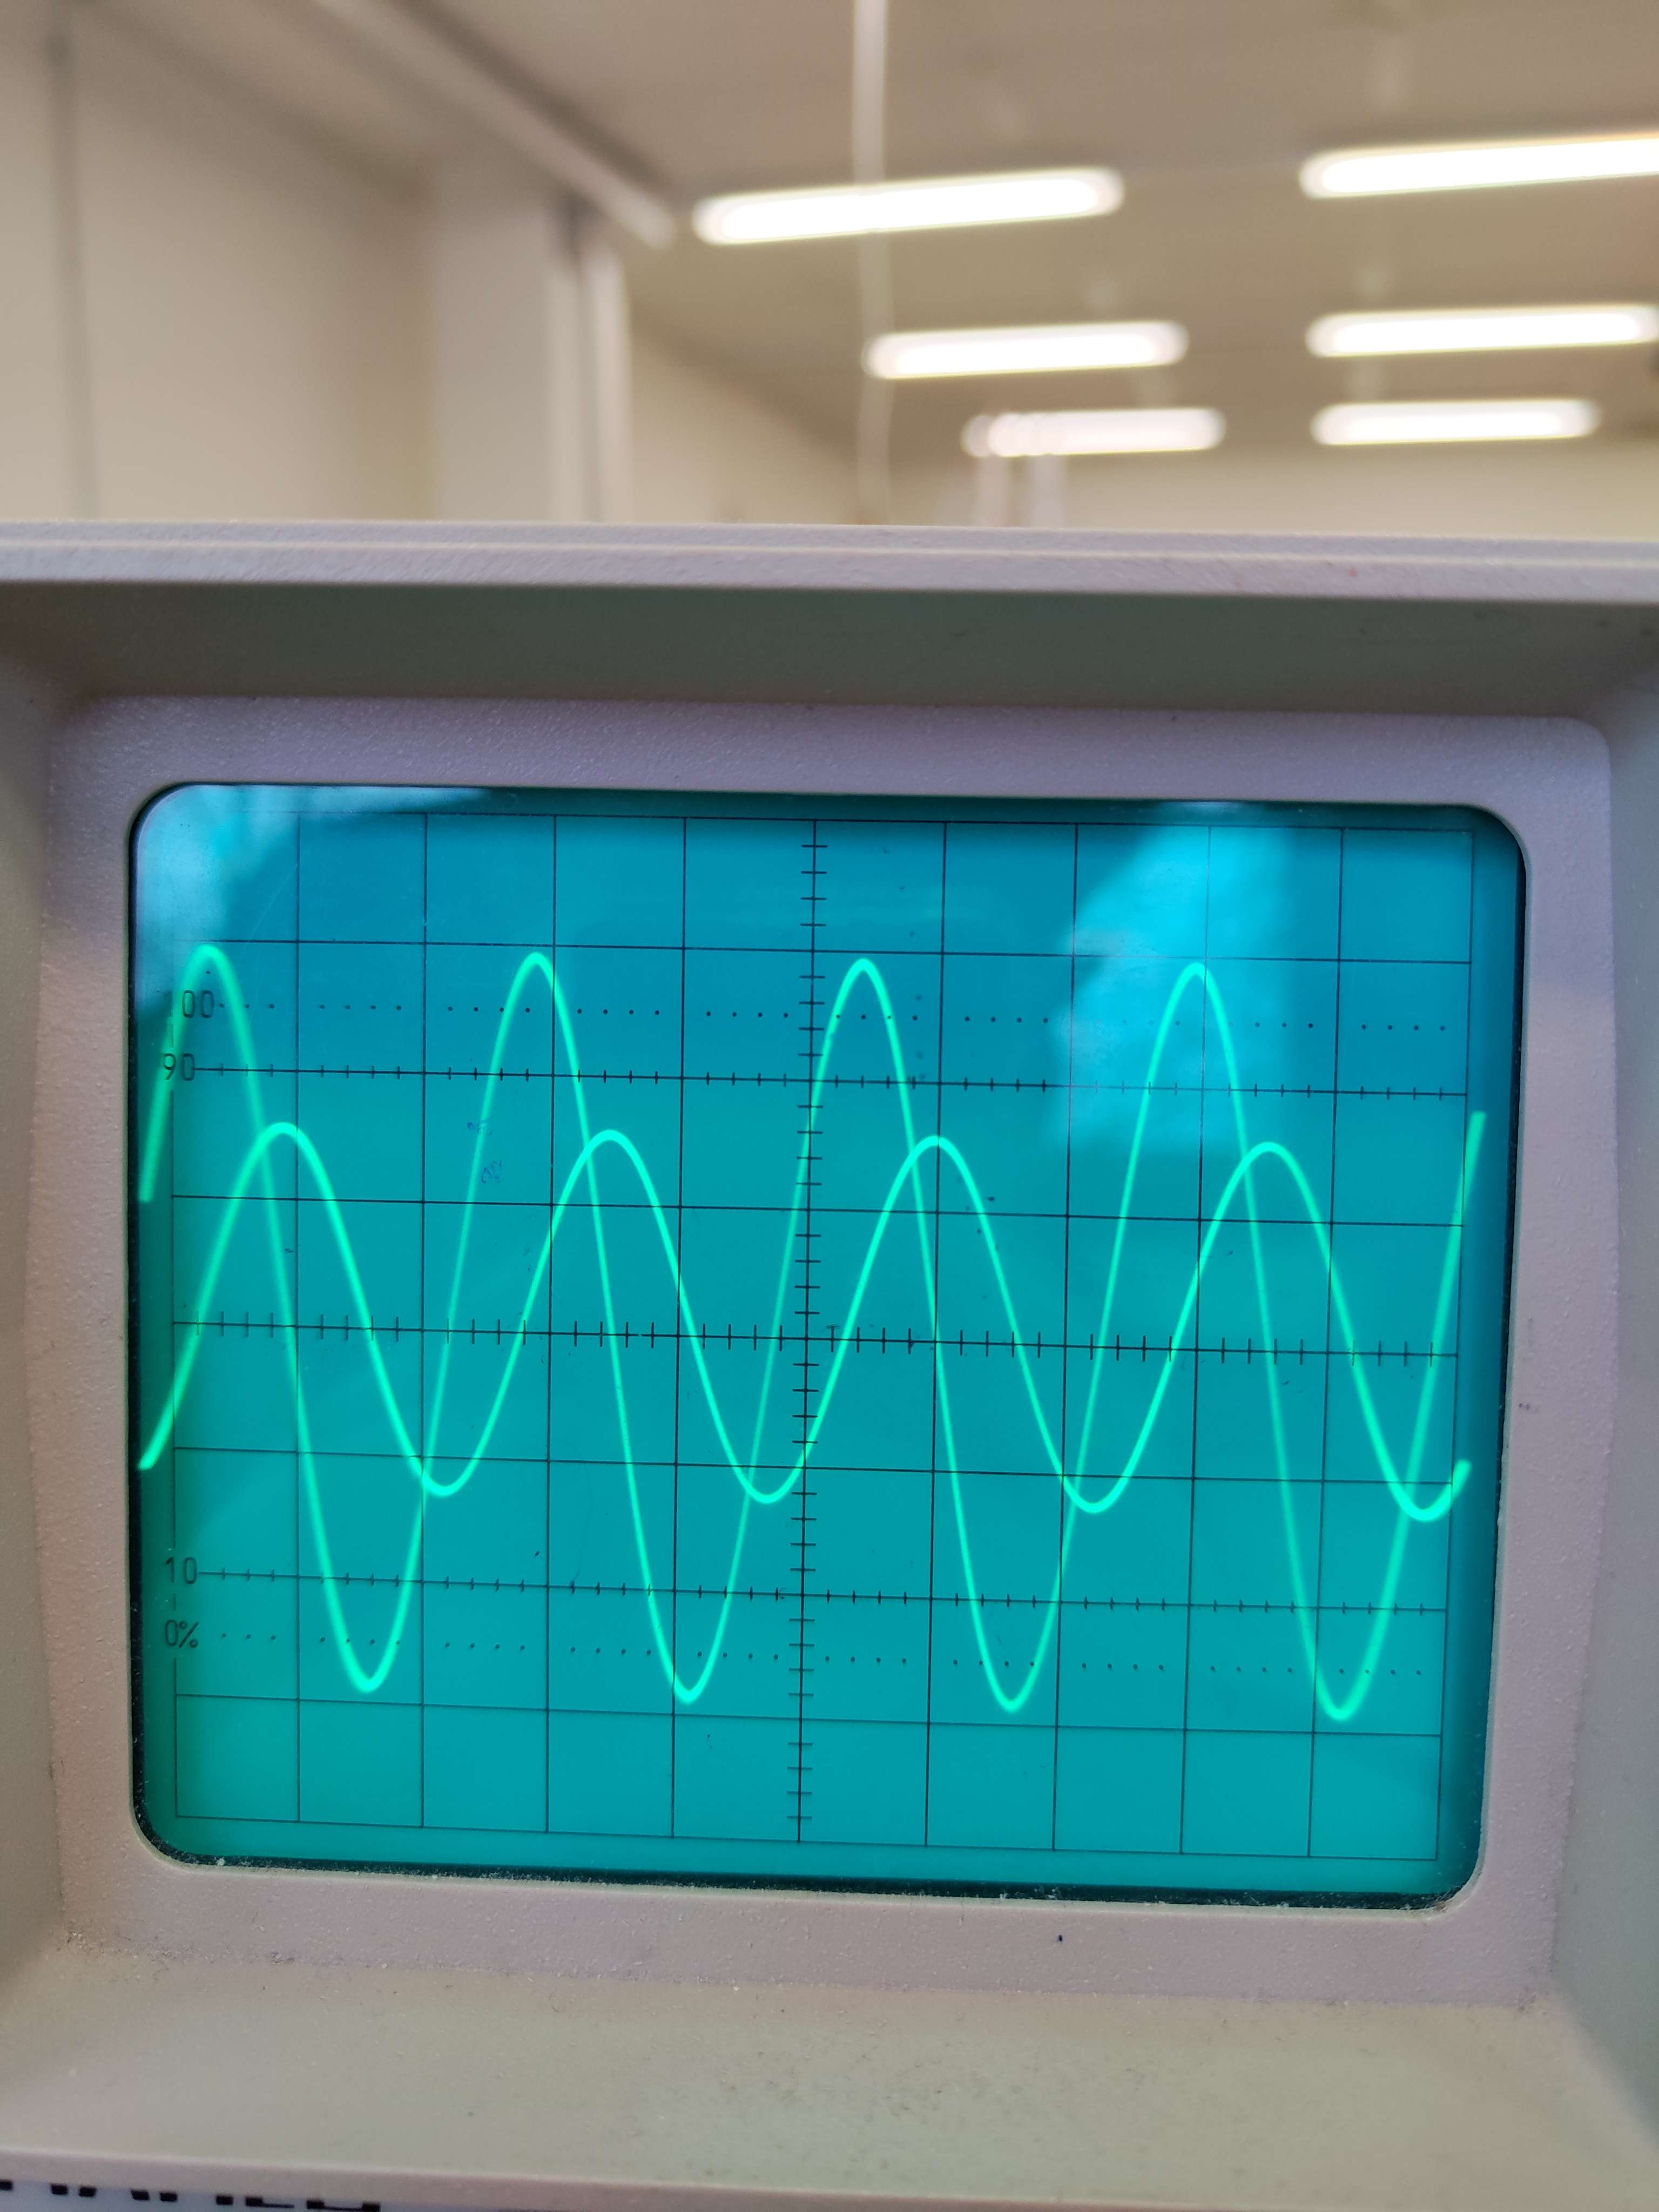
\includegraphics[height=3.3cm]{img/sinus.jpg}
        \caption{Sinus- und \\ Cosinusspannung}
        \label{fig:sinus}
    \end{subfigure}
    \begin{subfigure}{0.3\textwidth}
        \centering
        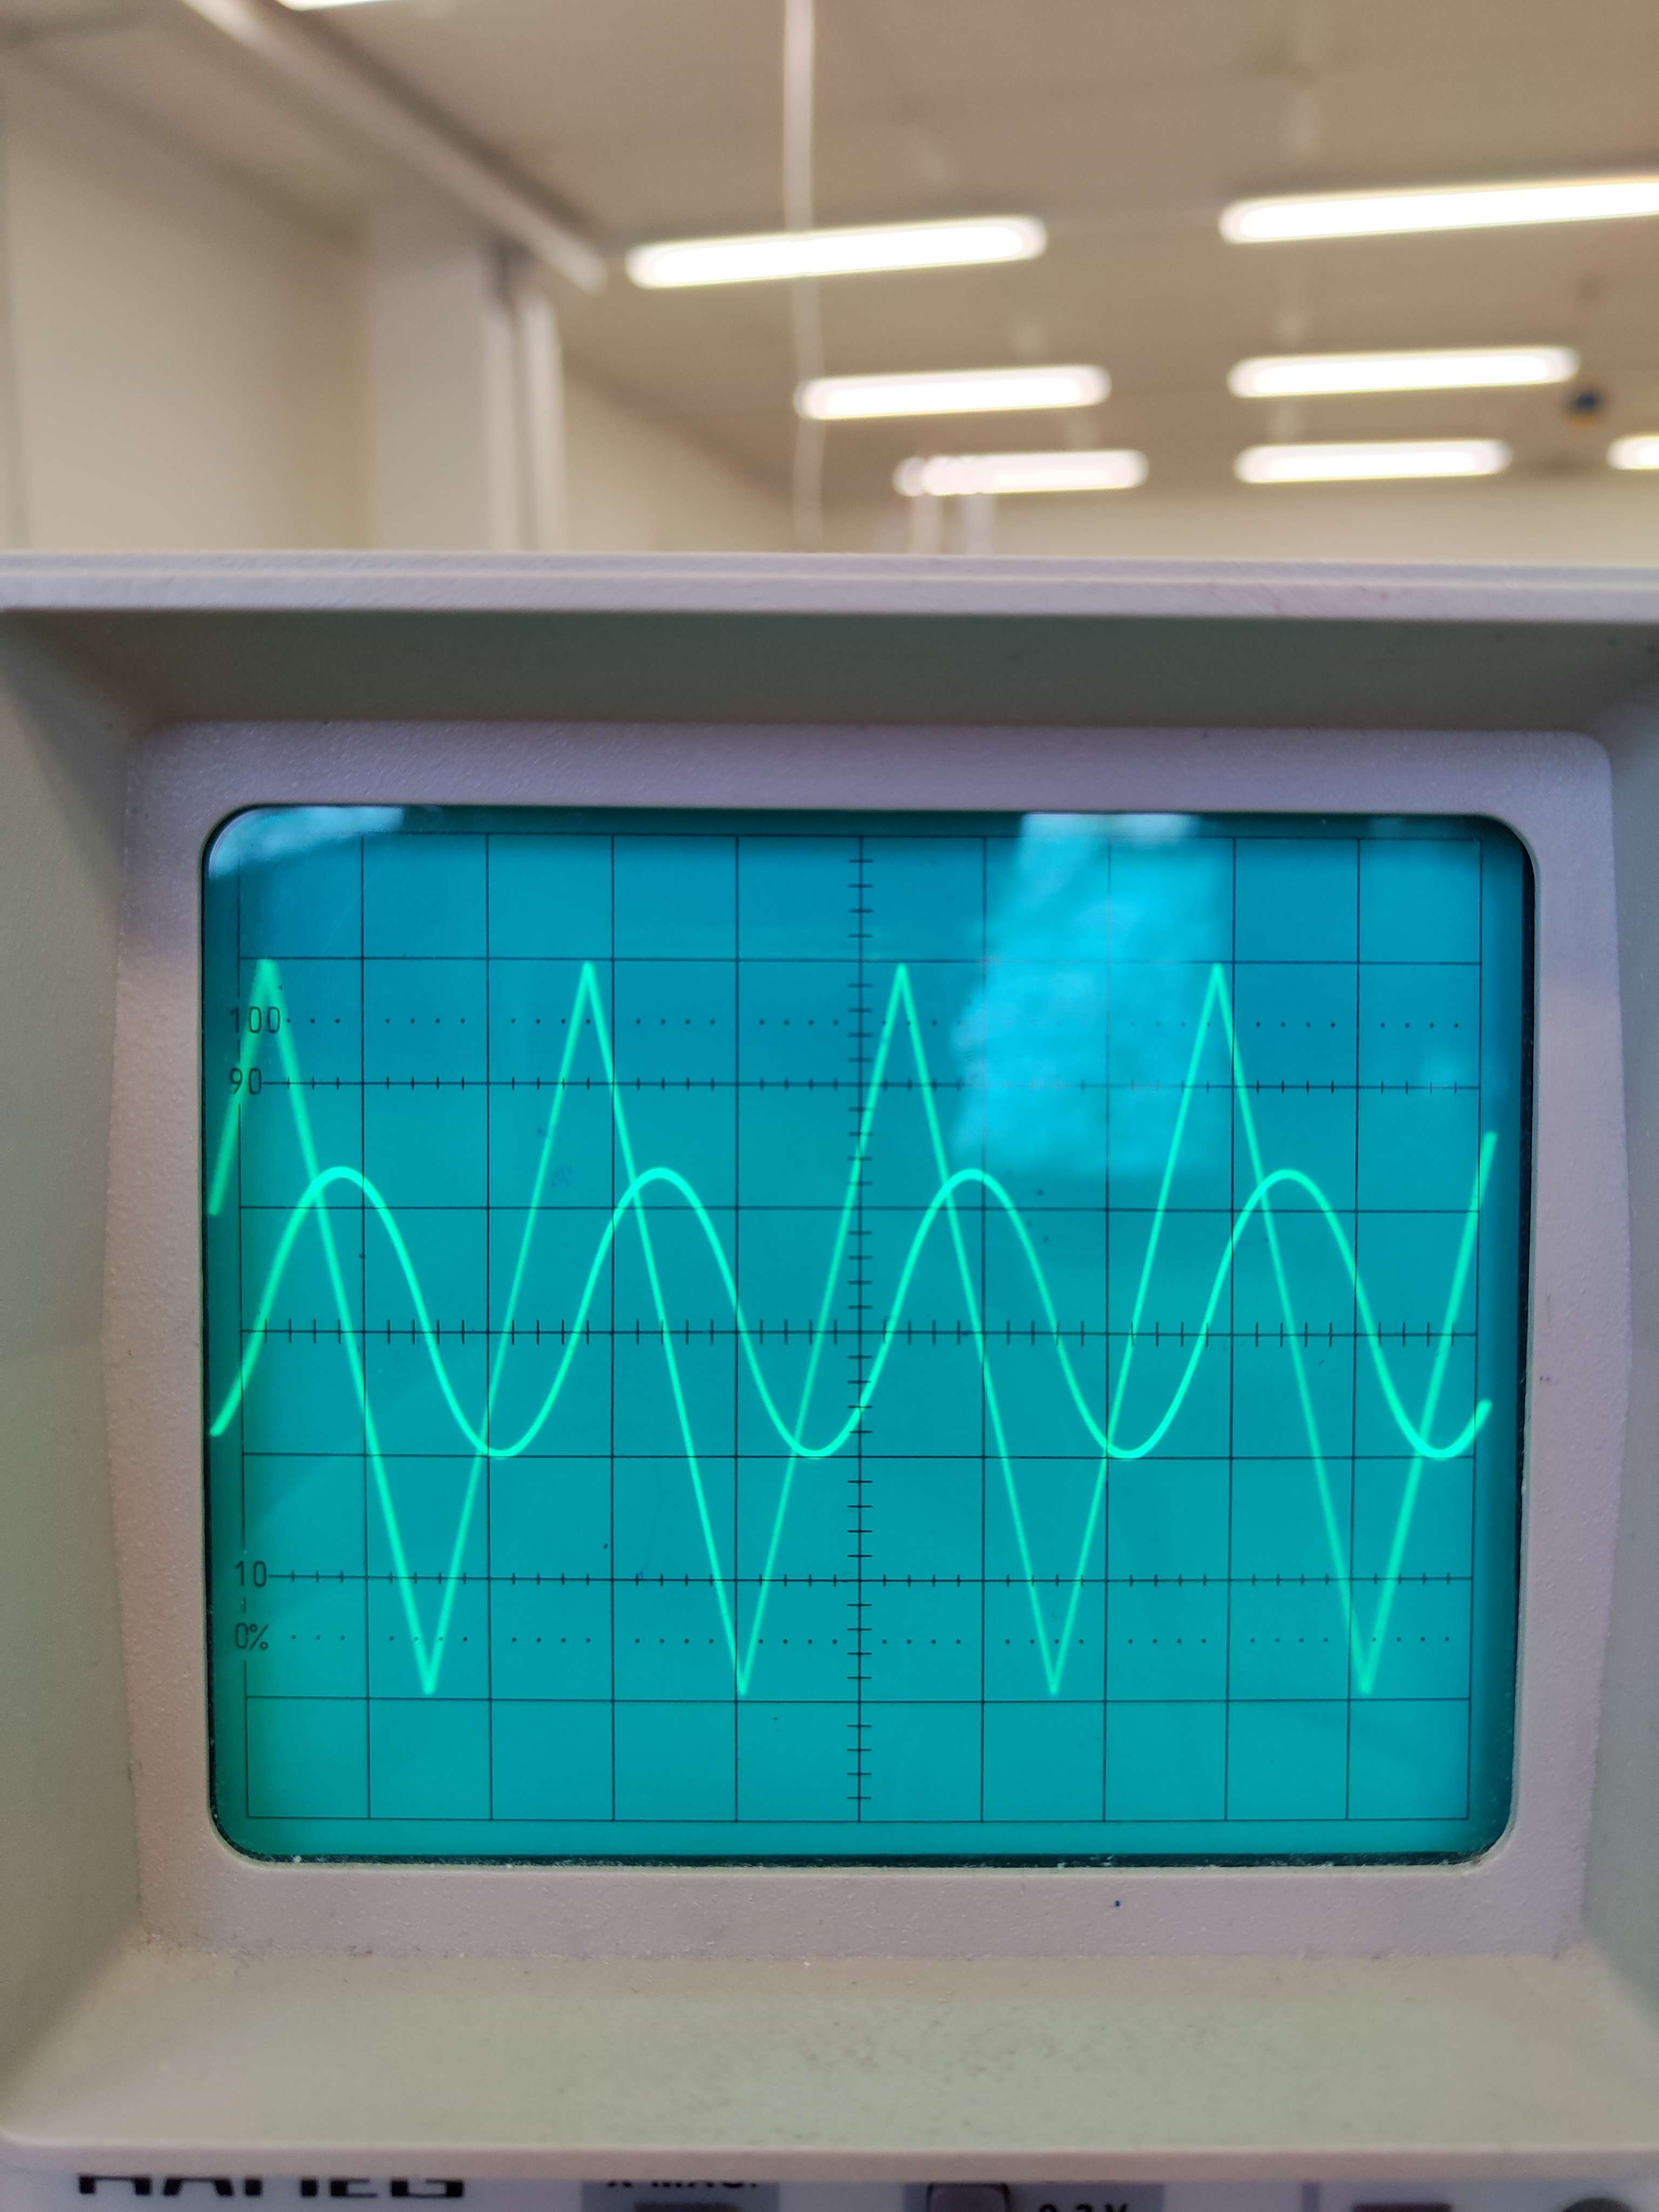
\includegraphics[height=3.3cm]{img/saegezahn.jpg}
        \caption{Sägezahn- und \\ Sinusspannung}
        \label{fig:saegezahn}
    \end{subfigure}
    \begin{subfigure}{0.3\textwidth}
        \centering
        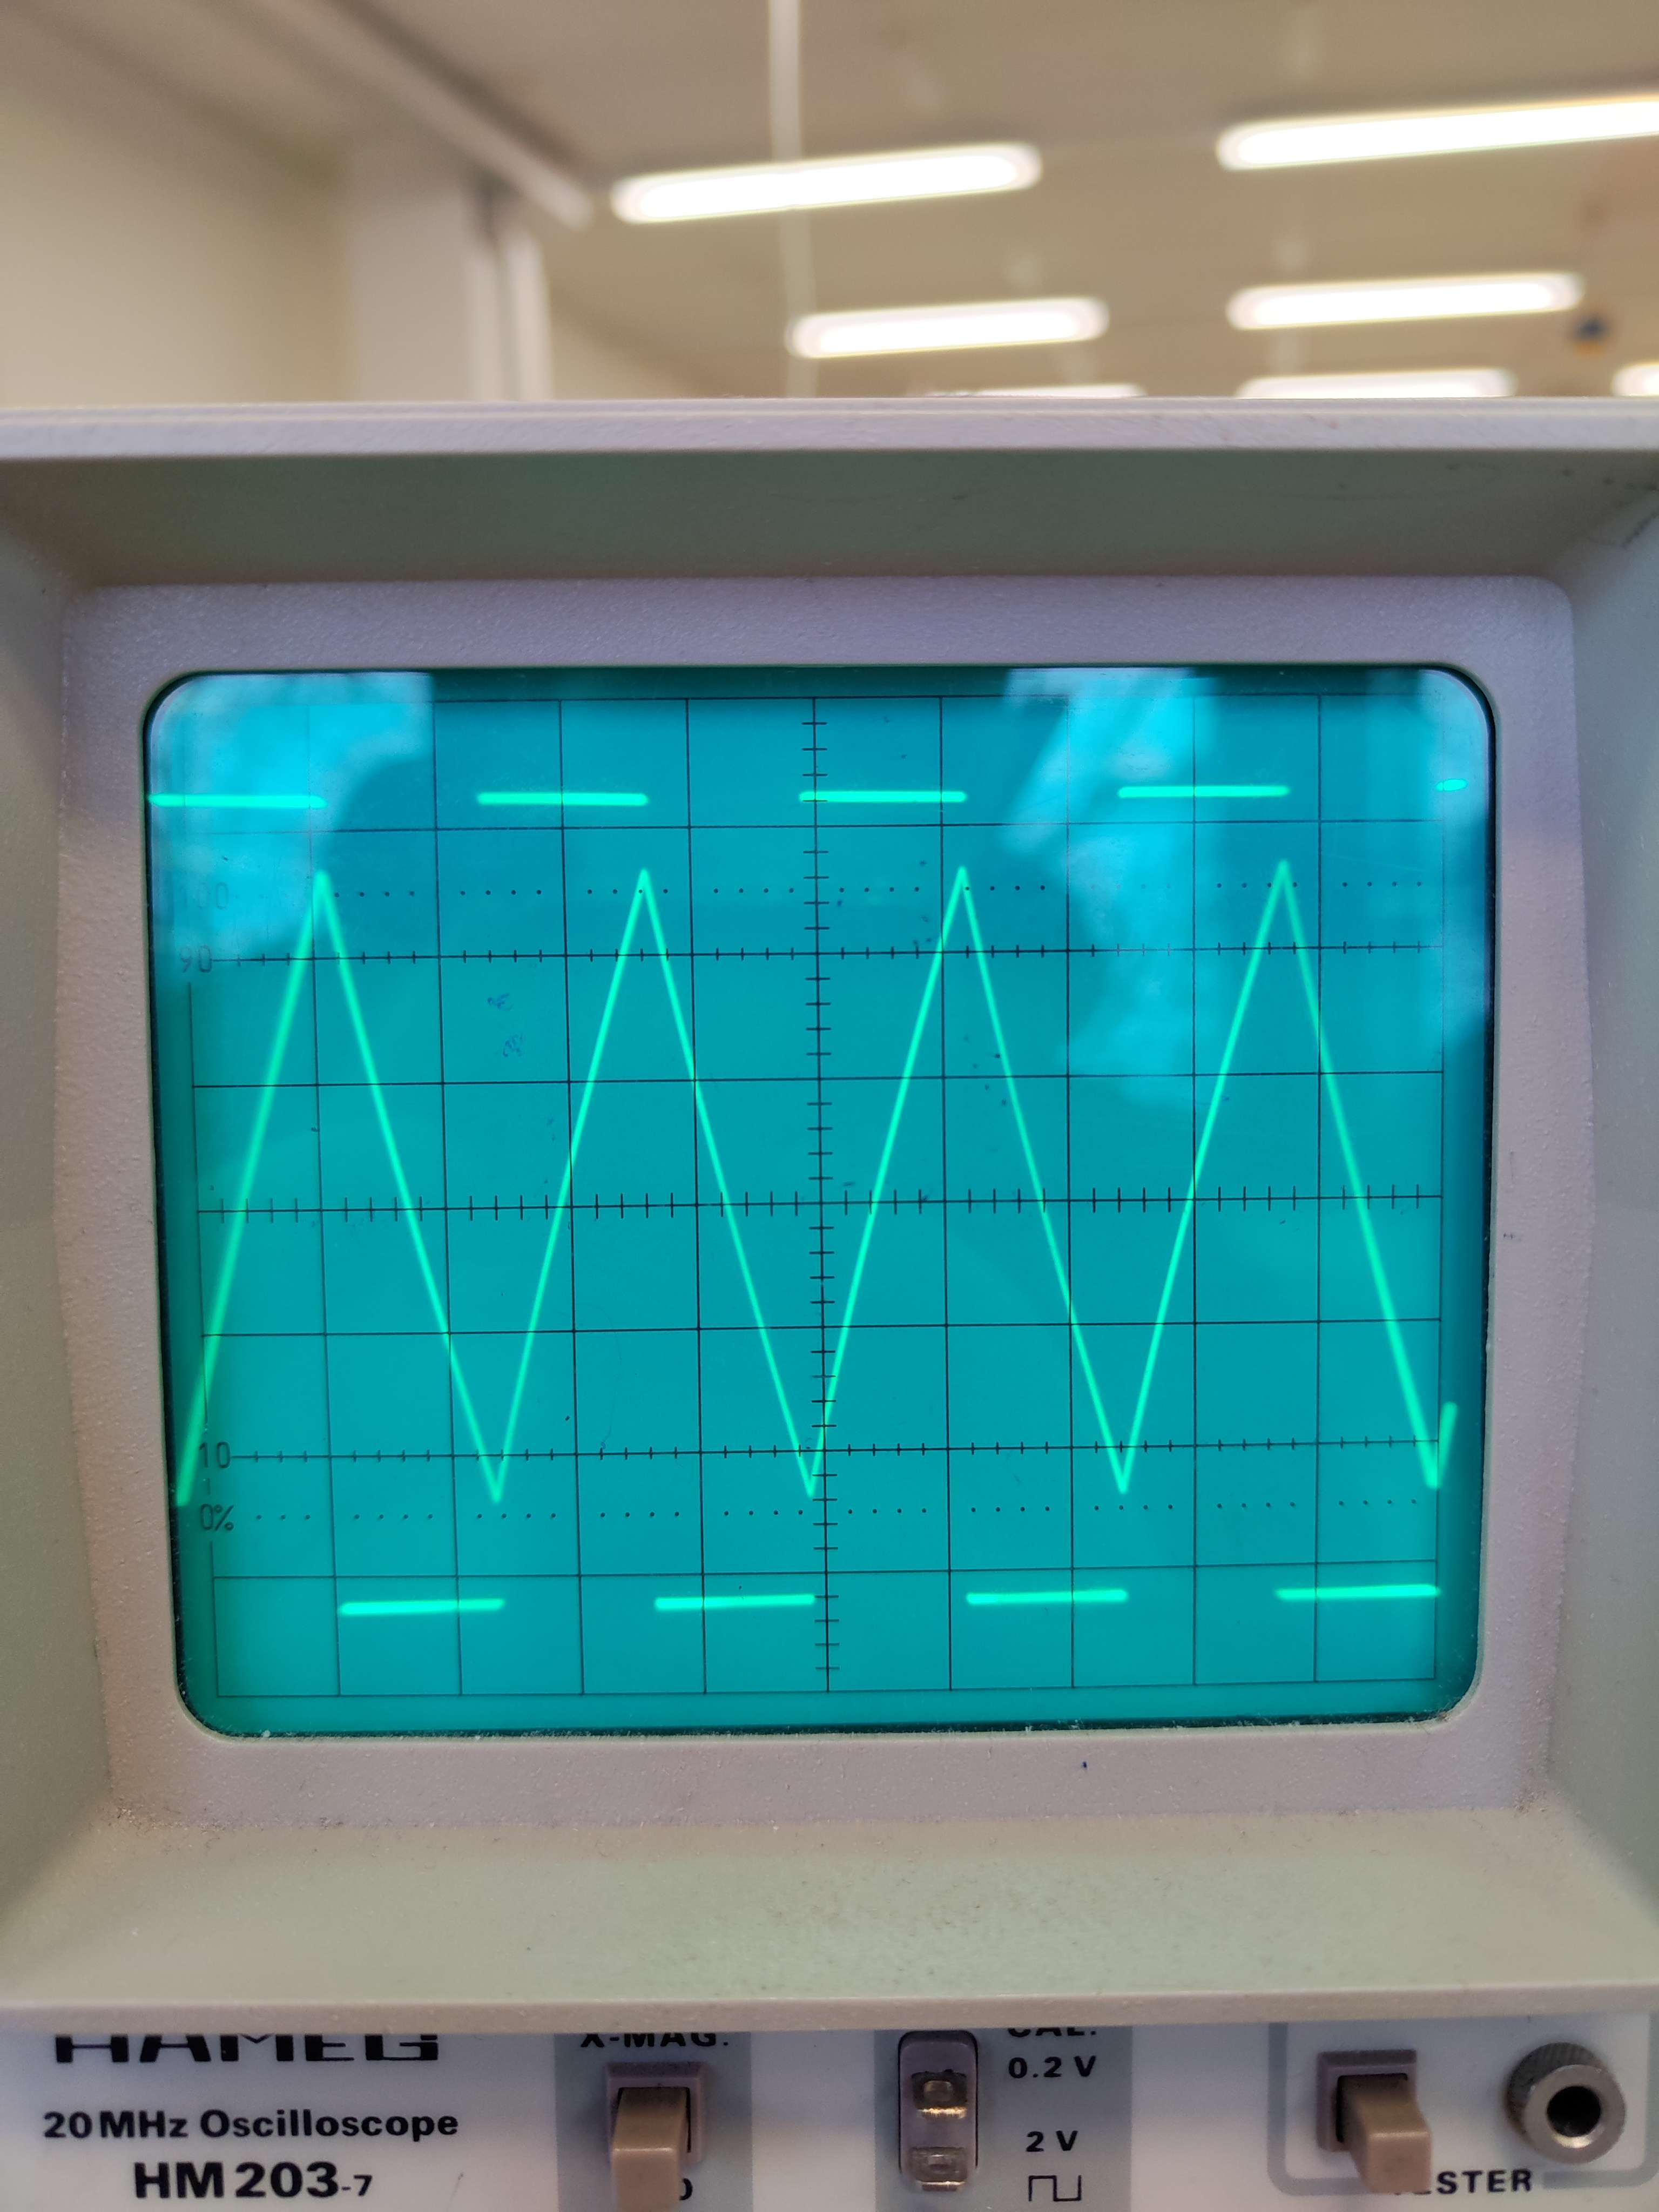
\includegraphics[height=3.3cm]{img/rechteck.jpg}
        \caption{Rechteck- und \\ Sägezahnspannung}
        \label{fig:rechteck}
    \end{subfigure}
    \caption{Fotos der Integratorschaltung für eine Generatorfrequenz von $\SI{792}{\hertz}$ und verschiedenen Generatorspannungen}
    \label{fig:integrator}
\end{figure}
\newpage